\documentclass[smallextended]{svjour3}
\usepackage[]{graphicx}\usepackage[]{xcolor}
% maxwidth is the original width if it is less than linewidth
% otherwise use linewidth (to make sure the graphics do not exceed the margin)
\makeatletter
\def\maxwidth{ %
  \ifdim\Gin@nat@width>\linewidth
    \linewidth
  \else
    \Gin@nat@width
  \fi
}
\makeatother

\definecolor{fgcolor}{rgb}{0.345, 0.345, 0.345}
\newcommand{\hlnum}[1]{\textcolor[rgb]{0.686,0.059,0.569}{#1}}%
\newcommand{\hlstr}[1]{\textcolor[rgb]{0.192,0.494,0.8}{#1}}%
\newcommand{\hlcom}[1]{\textcolor[rgb]{0.678,0.584,0.686}{\textit{#1}}}%
\newcommand{\hlopt}[1]{\textcolor[rgb]{0,0,0}{#1}}%
\newcommand{\hlstd}[1]{\textcolor[rgb]{0.345,0.345,0.345}{#1}}%
\newcommand{\hlkwa}[1]{\textcolor[rgb]{0.161,0.373,0.58}{\textbf{#1}}}%
\newcommand{\hlkwb}[1]{\textcolor[rgb]{0.69,0.353,0.396}{#1}}%
\newcommand{\hlkwc}[1]{\textcolor[rgb]{0.333,0.667,0.333}{#1}}%
\newcommand{\hlkwd}[1]{\textcolor[rgb]{0.737,0.353,0.396}{\textbf{#1}}}%
\let\hlipl\hlkwb

\usepackage{framed}
\makeatletter
\newenvironment{kframe}{%
 \def\at@end@of@kframe{}%
 \ifinner\ifhmode%
  \def\at@end@of@kframe{\end{minipage}}%
  \begin{minipage}{\columnwidth}%
 \fi\fi%
 \def\FrameCommand##1{\hskip\@totalleftmargin \hskip-\fboxsep
 \colorbox{shadecolor}{##1}\hskip-\fboxsep
     % There is no \\@totalrightmargin, so:
     \hskip-\linewidth \hskip-\@totalleftmargin \hskip\columnwidth}%
 \MakeFramed {\advance\hsize-\width
   \@totalleftmargin\z@ \linewidth\hsize
   \@setminipage}}%
 {\par\unskip\endMakeFramed%
 \at@end@of@kframe}
\makeatother

\definecolor{shadecolor}{rgb}{.97, .97, .97}
\definecolor{messagecolor}{rgb}{0, 0, 0}
\definecolor{warningcolor}{rgb}{1, 0, 1}
\definecolor{errorcolor}{rgb}{1, 0, 0}
\newenvironment{knitrout}{}{} % an empty environment to be redefined in TeX

\usepackage{alltt}
\newcommand{\SweaveOpts}[1]{}  % do not interfere with LaTeX
\newcommand{\SweaveInput}[1]{} % because they are not real TeX commands
\newcommand{\Sexpr}[1]{}       % will only be parsed by R

    
\smartqed  % flush right qed marks, e.g. at end of proof

\usepackage[colorlinks=true,linkcolor={blue},citecolor={blue},urlcolor={blue}]{hyperref}
%\usepackage{caption}
% Add longtable and ctable packages
\usepackage{longtable,ctable}
\usepackage{amsmath}
\usepackage{amssymb}
\usepackage{amsfonts}
\usepackage{multirow}
%\usepackage{amsthm}
\usepackage{graphicx}

\usepackage{booktabs}
%\usepackage{bookmark}

%\usepackage{caption}
%\usepackage{capt-of}

\usepackage{amsmath}
\usepackage{graphicx}
\usepackage{mathptmx}
\usepackage{natbib}

\usepackage{setspace}

%\usepackage{tikz-feynman}
%\usepackage{tikz} 
%\usetikzlibrary{positioning}
\usepackage[utf8]{inputenc}
\usepackage{pgf}


\usepackage{algorithm}
\usepackage{algpseudocode}
\usepackage{enumerate}

\usepackage{threeparttable}

\raggedbottom

\newcommand{\R}{R}
\newcommand{\gbsg}{gbsg}

%\def\FsNg{\hbox{FS}(M_{g})}

\def\FsNg{\hbox{FS-M}}

\def\hhat{\hat\theta(\hat{H})}
\def\hchat{\hat\theta(\hat{H}^{c})}
\def\hknow{\hat\theta(H)}
\def\hcknow{\hat\theta(H^{c})}
\def\hplim{\theta^{\dagger}(H)}
\def\hcplim{\theta^{\dagger}(H^{c})}

\def\sumin{\sum_{i=1}^n}
\def\nsumin{n^{-1}\sum_{i=1}^n}

\def\ns{n_{0}+n_{1}}
\def\na{n_{0}}
\def\nb{n_{1}}

\newcommand{\indep}{\perp \!\!\! \perp}

\textheight=9.25in \textwidth=6.0in 
\topmargin=0in
\evensidemargin=0in \oddsidemargin=0in



\begin{document}





\begin{knitrout}
\definecolor{shadecolor}{rgb}{0.969, 0.969, 0.969}\color{fgcolor}\begin{kframe}
\begin{alltt}
\hlkwd{rm}\hlstd{(}\hlkwc{list} \hlstd{=} \hlkwd{ls}\hlstd{())}

\hlcom{# Local github}
\hlstd{codepath} \hlkwb{<-} \hlkwd{c}\hlstd{(}\hlstr{"/media/larryleon/My Projects/GitHub/Forest-Search/R/"}\hlstd{)}
\hlkwd{source}\hlstd{(}\hlkwd{paste0}\hlstd{(codepath,} \hlstr{"source_forestsearch_v0.R"}\hlstd{))}
\hlkwd{source_fs_functions}\hlstd{(}\hlkwc{file_loc} \hlstd{= codepath)}

\hlkwd{library}\hlstd{(kableExtra)}
\hlkwd{library}\hlstd{(knitr)}
\hlkwd{library}\hlstd{(ggplot2)}
\hlkwd{library}\hlstd{(gridExtra)}
\hlkwd{library}\hlstd{(cubature)}
\hlkwd{library}\hlstd{(aVirtualTwins)}
\hlkwd{library}\hlstd{(randomForest)}
\hlkwd{library}\hlstd{(survival)}
\hlkwd{library}\hlstd{(survminer)}
\hlkwd{library}\hlstd{(grf)}
\hlkwd{library}\hlstd{(policytree)}
\hlkwd{library}\hlstd{(data.table)}
\hlkwd{library}\hlstd{(plyr)}
\hlkwd{library}\hlstd{(dplyr)}
\hlkwd{library}\hlstd{(glmnet)}
\hlkwd{library}\hlstd{(corrplot)}
\end{alltt}
\end{kframe}
\end{knitrout}




\begin{knitrout}
\definecolor{shadecolor}{rgb}{0.969, 0.969, 0.969}\color{fgcolor}\begin{kframe}
\begin{alltt}
\hlstd{maxFollow} \hlkwb{<-} \hlnum{84}
\hlstd{cens.type} \hlkwb{<-} \hlstr{"weibull"}

\hlcom{# m1 -censoring adjustment}
\hlstd{muC.adj} \hlkwb{<-} \hlkwd{log}\hlstd{(}\hlnum{1.5}\hlstd{)}
\hlstd{k.z3} \hlkwb{<-} \hlnum{1}
\hlstd{k.treat} \hlkwb{<-} \hlnum{0.9}

\hlstd{z1_frac} \hlkwb{<-} \hlnum{0.25}  \hlcom{# Default model index 'm1' (The 1st quartile of z1=er)}
\hlstd{pH_super} \hlkwb{<-} \hlnum{0.125}  \hlcom{# non-NULL re-defines z1_frac}

\hlkwa{if} \hlstd{(}\hlkwd{is.null}\hlstd{(pH_super)) \{}
    \hlcom{# pH_check<-with(gbsg,mean(pgr<=quantile(pgr,c(z3_frac),1,0) &}
    \hlcom{# er<=quantile(er,z1_frac)))}
    \hlstd{pH_check} \hlkwb{<-} \hlkwd{with}\hlstd{(gbsg,} \hlkwd{mean}\hlstd{(meno} \hlopt{==} \hlnum{0} \hlopt{&} \hlstd{er} \hlopt{<=} \hlkwd{quantile}\hlstd{(er, z1_frac)))}
    \hlkwd{cat}\hlstd{(}\hlstr{"Underlying pH_super"}\hlstd{,} \hlkwd{c}\hlstd{(pH_check),} \hlstr{"\textbackslash{}n"}\hlstd{)}
\hlstd{\}}
\hlcom{# pH_super specified If pH_super then override z1_frac and find z1_frac to}
\hlcom{# yield pH_super}

\hlkwa{if} \hlstd{(}\hlopt{!}\hlkwd{is.null}\hlstd{(pH_super)) \{}
    \hlcom{# Approximate Z1 quantile to yield pH proportion}
    \hlstd{z1_q} \hlkwb{<-} \hlkwd{uniroot}\hlstd{(propH.obj4,} \hlkwd{c}\hlstd{(}\hlnum{0}\hlstd{,} \hlnum{1}\hlstd{),} \hlkwc{tol} \hlstd{=} \hlnum{1e-04}\hlstd{,} \hlkwc{pH.target} \hlstd{= pH_super)}\hlopt{$}\hlstd{root}
    \hlcom{# pH_check<-with(gbsg,mean(pgr<=quantile(pgr,c(z3_frac),1,0) &}
    \hlcom{# er<=quantile(er,z1_q)))}
    \hlstd{pH_check} \hlkwb{<-} \hlkwd{with}\hlstd{(gbsg,} \hlkwd{mean}\hlstd{(meno} \hlopt{==} \hlnum{0} \hlopt{&} \hlstd{er} \hlopt{<=} \hlkwd{quantile}\hlstd{(er, z1_q)))}
    \hlkwd{cat}\hlstd{(}\hlstr{"pH"}\hlstd{,} \hlkwd{c}\hlstd{(pH_check),} \hlstr{"\textbackslash{}n"}\hlstd{)}
    \hlstd{rel_error} \hlkwb{<-} \hlstd{(pH_super} \hlopt{-} \hlstd{pH_check)}\hlopt{/}\hlstd{pH_super}
    \hlkwa{if} \hlstd{(}\hlkwd{abs}\hlstd{(rel_error)} \hlopt{>=} \hlnum{0.1}\hlstd{)}
        \hlkwd{stop}\hlstd{(}\hlstr{"pH_super approximation relative error exceeds 10%"}\hlstd{)}
    \hlstd{z1_frac} \hlkwb{<-} \hlstd{z1_q}
    \hlkwd{cat}\hlstd{(}\hlstr{"Underlying pH_super"}\hlstd{,} \hlkwd{c}\hlstd{(pH_check),} \hlstr{"\textbackslash{}n"}\hlstd{)}
\hlstd{\}}
\end{alltt}
\begin{verbatim}
## pH 0.122449 
## Underlying pH_super 0.122449
\end{verbatim}
\begin{alltt}
\hlcom{# Bootstrap on log(hr) scale converted to HR (est.loghr=TRUE & est.scale='hr')}
\hlstd{t.start.all} \hlkwb{<-} \hlkwd{proc.time}\hlstd{()[}\hlnum{3}\hlstd{]}
\end{alltt}
\end{kframe}
\end{knitrout}


\begin{knitrout}
\definecolor{shadecolor}{rgb}{0.969, 0.969, 0.969}\color{fgcolor}\begin{kframe}
\begin{alltt}
\hlcom{######################### Forest search criteria}
\hlstd{hr.threshold} \hlkwb{<-} \hlnum{1.25}  \hlcom{# Initital candidates }
\hlstd{hr.consistency} \hlkwb{<-} \hlnum{1}  \hlcom{# Candidates for many splits}
\hlstd{pconsistency.threshold} \hlkwb{<-} \hlnum{0.9}
\hlstd{stop.threshold} \hlkwb{<-} \hlnum{0.95}
\hlstd{maxk} \hlkwb{<-} \hlnum{2}
\hlstd{nmin.fs} \hlkwb{<-} \hlnum{60}
\hlstd{pstop_futile} \hlkwb{<-} \hlnum{0.5}
\hlcom{# Limit timing for forestsearch}
\hlstd{max.minutes} \hlkwb{<-} \hlnum{3}
\hlstd{m1.threshold} \hlkwb{<-} \hlnum{Inf}  \hlcom{# Turning this off (Default)}
\hlcom{# pconsistency.threshold<-0.70 # Minimum threshold (will choose max among}
\hlcom{# subgroups satisfying)}
\hlstd{fs.splits} \hlkwb{<-} \hlnum{400}  \hlcom{# How many times to split for consistency}
\hlcom{# vi is % factor is selected in cross-validation --> higher more important}
\hlstd{vi.grf.min} \hlkwb{<-} \hlnum{0.2}
\hlcom{# Null, turns off grf screening}
\hlstd{d.min} \hlkwb{<-} \hlnum{10}  \hlcom{# Min number of events for both arms (d0.min=d1.min=d.min)}
\hlcom{# default=5 Virtual twins analysis Counter-factual difference (C-E) >=}
\hlcom{# vt.threshold Large values in favor of C (control)}
\hlstd{vt.threshold} \hlkwb{<-} \hlnum{0.225}  \hlcom{# For VT delta}
\hlstd{treat.threshold} \hlkwb{<-} \hlnum{0}

\hlstd{maxdepth} \hlkwb{<-} \hlnum{2}
\hlstd{n.min} \hlkwb{<-} \hlnum{60}
\hlstd{ntree} \hlkwb{<-} \hlnum{1000}
\hlcom{# GRF criteria}
\hlstd{dmin.grf} \hlkwb{<-} \hlnum{12}  \hlcom{# For GRF delta}
\hlcom{# Note: For CRT this represents dmin.grf/2 RMS for control (-dmin.grf/2 for}
\hlcom{# treatment)}
\hlstd{frac.tau} \hlkwb{<-} \hlnum{0.6}

\hlstd{outcome.name} \hlkwb{<-} \hlkwd{c}\hlstd{(}\hlstr{"y.sim"}\hlstd{)}
\hlstd{event.name} \hlkwb{<-} \hlkwd{c}\hlstd{(}\hlstr{"event.sim"}\hlstd{)}
\hlstd{id.name} \hlkwb{<-} \hlkwd{c}\hlstd{(}\hlstr{"id"}\hlstd{)}
\hlstd{treat.name} \hlkwb{<-} \hlkwd{c}\hlstd{(}\hlstr{"treat"}\hlstd{)}

\hlstd{cox.formula.sim} \hlkwb{<-} \hlkwd{as.formula}\hlstd{(}\hlkwd{paste}\hlstd{(}\hlstr{"Surv(y.sim,event.sim)~treat"}\hlstd{))}
\hlstd{cox.formula.adj.sim} \hlkwb{<-} \hlkwd{as.formula}\hlstd{(}\hlkwd{paste}\hlstd{(}\hlstr{"Surv(y.sim,event.sim)~treat+v1+v2+v3+v4+v5"}\hlstd{))}
\end{alltt}
\end{kframe}
\end{knitrout}



\begin{knitrout}
\definecolor{shadecolor}{rgb}{0.969, 0.969, 0.969}\color{fgcolor}\begin{kframe}
\begin{alltt}
\hlstd{mod.harm} \hlkwb{<-} \hlstr{"alt"}
\hlstd{hrH.target} \hlkwb{<-} \hlnum{2.5}
\hlcom{# out.loc = NULL turns off file creation}
\hlstd{N} \hlkwb{<-} \hlnum{700}
\hlstd{this.dgm} \hlkwb{<-} \hlkwd{get.dgm4}\hlstd{(}\hlkwc{mod.harm} \hlstd{= mod.harm,} \hlkwc{N} \hlstd{= N,} \hlkwc{k.treat} \hlstd{= k.treat,} \hlkwc{hrH.target} \hlstd{= hrH.target,}
    \hlkwc{cens.type} \hlstd{= cens.type,} \hlkwc{out.loc} \hlstd{=} \hlkwa{NULL}\hlstd{,} \hlkwc{details} \hlstd{=} \hlnum{TRUE}\hlstd{,} \hlkwc{parms_torand} \hlstd{=} \hlnum{FALSE}\hlstd{)}
\end{alltt}
\end{kframe}
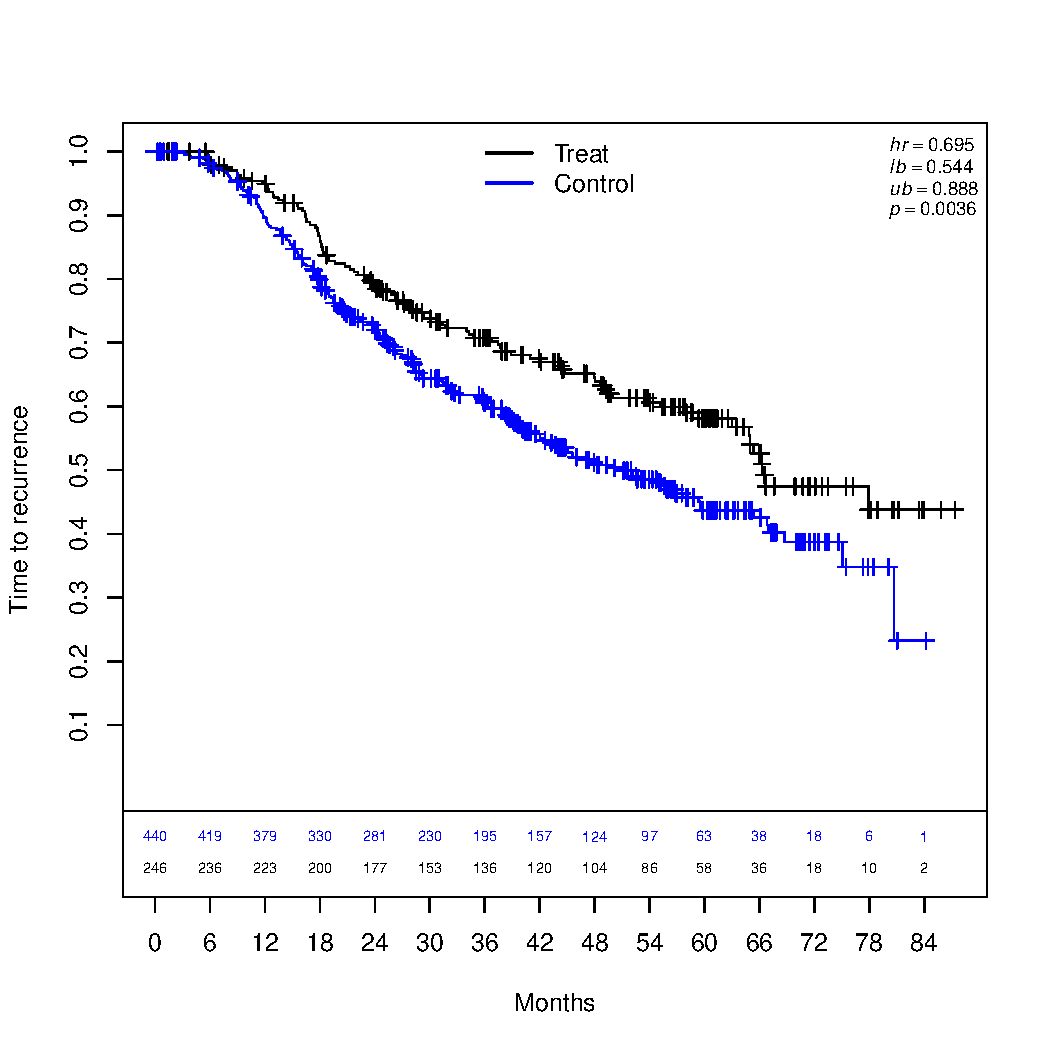
\includegraphics[width=\maxwidth]{figure/r_DGMsetup-1} 
\begin{kframe}\begin{verbatim}
## Super-population empirical harm and non-harm hazard ratios= 2.499996 0.6466405 
## Causal HR (empirical ITT)= 0.7125876
\end{verbatim}
\end{kframe}
\end{knitrout}

\begin{knitrout}
\definecolor{shadecolor}{rgb}{0.969, 0.969, 0.969}\color{fgcolor}\begin{kframe}
\begin{alltt}
\hlstd{file_out} \hlkwb{<-} \hlkwd{c}\hlstd{(}\hlstr{"output/sim-FS4_Lasso_ex11.Rdata"}\hlstd{)}

\hlstd{n_add_noise} \hlkwb{<-} \hlnum{3}

\hlstd{sim} \hlkwb{<-} \hlnum{23}

\hlstd{dgm} \hlkwb{<-} \hlstd{this.dgm}\hlopt{$}\hlstd{dgm}

\hlstd{x} \hlkwb{<-} \hlkwd{sim_aftm4_gbsg}\hlstd{(}\hlkwc{dgm} \hlstd{= dgm,} \hlkwc{n} \hlstd{= N,} \hlkwc{maxFollow} \hlstd{= maxFollow,} \hlkwc{muC.adj} \hlstd{= muC.adj,} \hlkwc{simid} \hlstd{= sim)}

\hlstd{kmfit} \hlkwb{<-} \hlkwd{survfit}\hlstd{(}\hlkwd{Surv}\hlstd{(y.sim, event)} \hlopt{~} \hlstd{treat,} \hlkwc{data} \hlstd{= x)}

\hlkwd{ggsurvplot}\hlstd{(kmfit,} \hlkwc{data} \hlstd{= x,} \hlkwc{main} \hlstd{=} \hlstr{"K-M curves for simulated data"}\hlstd{,} \hlkwc{legend} \hlstd{=} \hlstr{"top"}\hlstd{,}
    \hlkwc{legend.title} \hlstd{=} \hlstr{"Treatment"}\hlstd{,} \hlkwc{legend.labs} \hlstd{=} \hlkwd{c}\hlstd{(}\hlstr{"Control"}\hlstd{,} \hlstr{"Experimental"}\hlstd{),} \hlkwc{palette} \hlstd{=} \hlstr{"grey"}\hlstd{,}
    \hlkwc{risk.table} \hlstd{=} \hlnum{TRUE}\hlstd{,} \hlkwc{risk.table.col} \hlstd{=} \hlstr{"strata"}\hlstd{)}
\end{alltt}
\end{kframe}
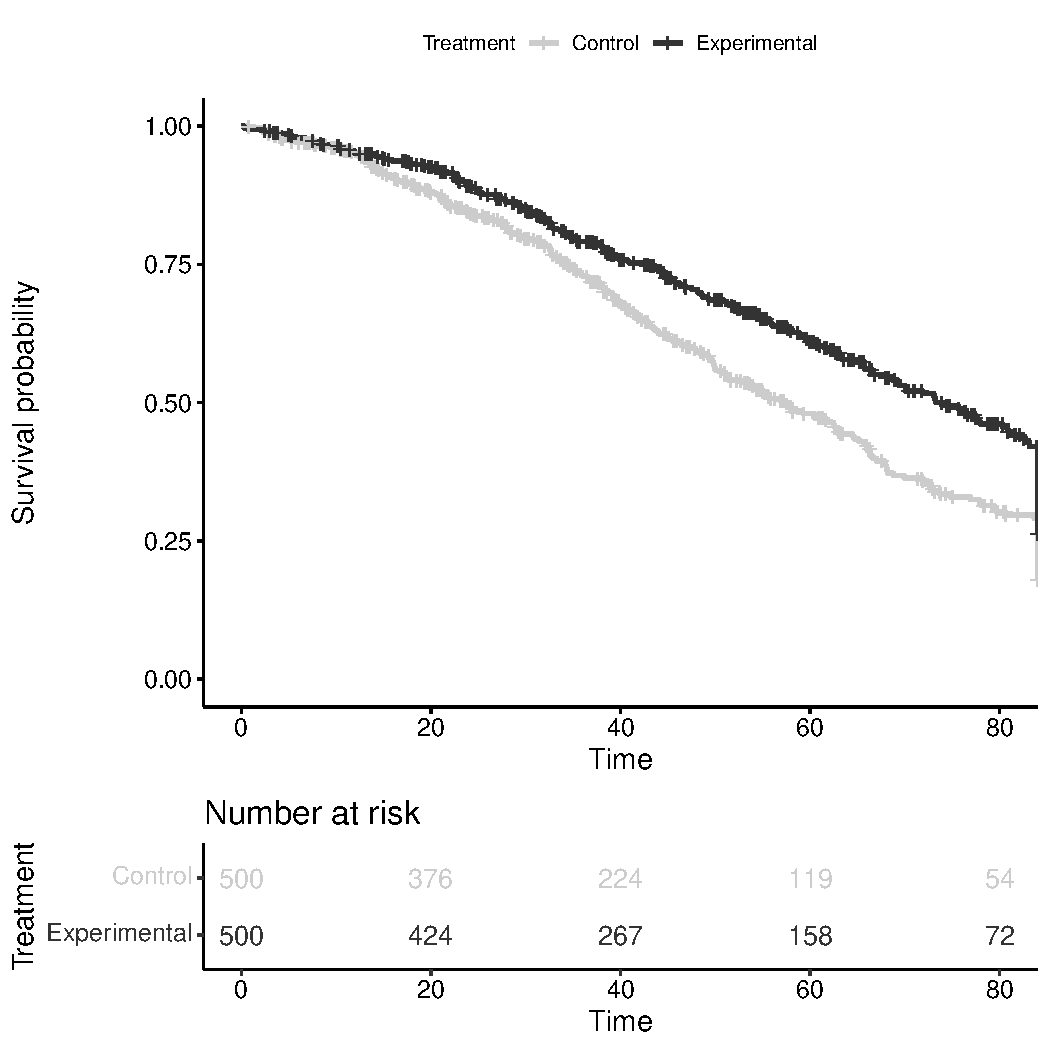
\includegraphics[width=\maxwidth]{figure/r_FSanalysis-1} 
\begin{kframe}\begin{alltt}
\hlkwa{if} \hlstd{(n_add_noise} \hlopt{==} \hlnum{0}\hlstd{) \{}
    \hlstd{confounders.name} \hlkwb{<-} \hlkwd{c}\hlstd{(}\hlstr{"z1"}\hlstd{,} \hlstr{"z2"}\hlstd{,} \hlstr{"z3"}\hlstd{,} \hlstr{"z4"}\hlstd{,} \hlstr{"z5"}\hlstd{,} \hlstr{"size"}\hlstd{,} \hlstr{"grade3"}\hlstd{)}
\hlstd{\}}

\hlkwa{if} \hlstd{(n_add_noise} \hlopt{==} \hlnum{5}\hlstd{) \{}
    \hlkwd{set.seed}\hlstd{(}\hlnum{8316951} \hlopt{+} \hlnum{1000} \hlopt{*} \hlstd{sim)}
    \hlcom{# Add 5 noise}
    \hlstd{x}\hlopt{$}\hlstd{noise1} \hlkwb{<-} \hlkwd{rnorm}\hlstd{(N)}
    \hlstd{x}\hlopt{$}\hlstd{noise2} \hlkwb{<-} \hlkwd{rnorm}\hlstd{(N)}
    \hlstd{x}\hlopt{$}\hlstd{noise3} \hlkwb{<-} \hlkwd{rnorm}\hlstd{(N)}
    \hlstd{x}\hlopt{$}\hlstd{noise4} \hlkwb{<-} \hlkwd{rnorm}\hlstd{(N)}
    \hlstd{x}\hlopt{$}\hlstd{noise5} \hlkwb{<-} \hlkwd{rnorm}\hlstd{(N)}
    \hlstd{confounders.name} \hlkwb{<-} \hlkwd{c}\hlstd{(}\hlstr{"z1"}\hlstd{,} \hlstr{"z2"}\hlstd{,} \hlstr{"z3"}\hlstd{,} \hlstr{"z4"}\hlstd{,} \hlstr{"z5"}\hlstd{,} \hlstr{"size"}\hlstd{,} \hlstr{"grade3"}\hlstd{,} \hlstr{"noise1"}\hlstd{,}
        \hlstr{"noise2"}\hlstd{,} \hlstr{"noise3"}\hlstd{,} \hlstr{"noise4"}\hlstd{,} \hlstr{"noise5"}\hlstd{)}
\hlstd{\}}

\hlkwa{if} \hlstd{(n_add_noise} \hlopt{==} \hlnum{3}\hlstd{) \{}
    \hlkwd{set.seed}\hlstd{(}\hlnum{8316951} \hlopt{+} \hlnum{1000} \hlopt{*} \hlstd{sim)}
    \hlcom{# Add 3 noise}
    \hlstd{x}\hlopt{$}\hlstd{noise1} \hlkwb{<-} \hlkwd{rnorm}\hlstd{(N,} \hlkwc{sd} \hlstd{=} \hlnum{1}\hlstd{)}
    \hlstd{x}\hlopt{$}\hlstd{noise2} \hlkwb{<-} \hlkwd{rnorm}\hlstd{(N,} \hlkwc{sd} \hlstd{=} \hlnum{1}\hlstd{)}
    \hlstd{x}\hlopt{$}\hlstd{noise3} \hlkwb{<-} \hlkwd{rnorm}\hlstd{(N,} \hlkwc{sd} \hlstd{=} \hlnum{1}\hlstd{)}
    \hlstd{confounders.name} \hlkwb{<-} \hlkwd{c}\hlstd{(}\hlstr{"z1"}\hlstd{,} \hlstr{"z2"}\hlstd{,} \hlstr{"z3"}\hlstd{,} \hlstr{"z4"}\hlstd{,} \hlstr{"z5"}\hlstd{,} \hlstr{"size"}\hlstd{,} \hlstr{"grade3"}\hlstd{,} \hlstr{"noise1"}\hlstd{,}
        \hlstr{"noise2"}\hlstd{,} \hlstr{"noise3"}\hlstd{)}
\hlstd{\}}

\hlcom{# More challenging which_replace <- which(confounders.name=='z1')}
\hlcom{# confounders.name[which_replace] <- 'er'}

\hlstd{cox.formula.check} \hlkwb{<-} \hlkwd{as.formula}\hlstd{(}\hlkwd{paste}\hlstd{(}\hlstr{"Surv(y.sim,event.sim)~treat+v1+v2+v3+v4+v5+size+grade3+noise1+noise2+noise3"}\hlstd{))}
\hlkwd{coxph}\hlstd{(cox.formula.check,} \hlkwc{data} \hlstd{= x)}
\end{alltt}
\begin{verbatim}
## Call:
## coxph(formula = cox.formula.check, data = x)
## 
##              coef  exp(coef)   se(coef)      z        p
## treat  -4.288e-01  6.513e-01  1.088e-01 -3.941 8.12e-05
## v11     7.018e-02  1.073e+00  1.274e-01  0.551   0.5817
## v21    -3.014e-01  7.398e-01  1.680e-01 -1.795   0.0727
## v31     3.932e-01  1.482e+00  1.689e-01  2.328   0.0199
## v41     8.918e-01  2.439e+00  1.206e-01  7.392 1.44e-13
## v51    -1.047e+00  3.509e-01  1.126e-01 -9.303  < 2e-16
## size   -4.146e-06  1.000e+00  3.407e-03 -0.001   0.9990
## grade3 -1.816e-01  8.339e-01  1.252e-01 -1.450   0.1470
## noise1  2.406e-02  1.024e+00  5.405e-02  0.445   0.6562
## noise2 -4.244e-02  9.585e-01  5.610e-02 -0.756   0.4494
## noise3  5.278e-02  1.054e+00  5.763e-02  0.916   0.3598
## 
## Likelihood ratio test=171.6  on 11 df, p=< 2.2e-16
## n= 700, number of events= 372
\end{verbatim}
\begin{alltt}
\hlstd{Zm} \hlkwb{<-} \hlkwd{cor}\hlstd{(}\hlkwd{as.matrix}\hlstd{(x[,} \hlkwd{c}\hlstd{(confounders.name)]))}
\hlkwd{corrplot}\hlstd{(Zm)}
\end{alltt}
\end{kframe}
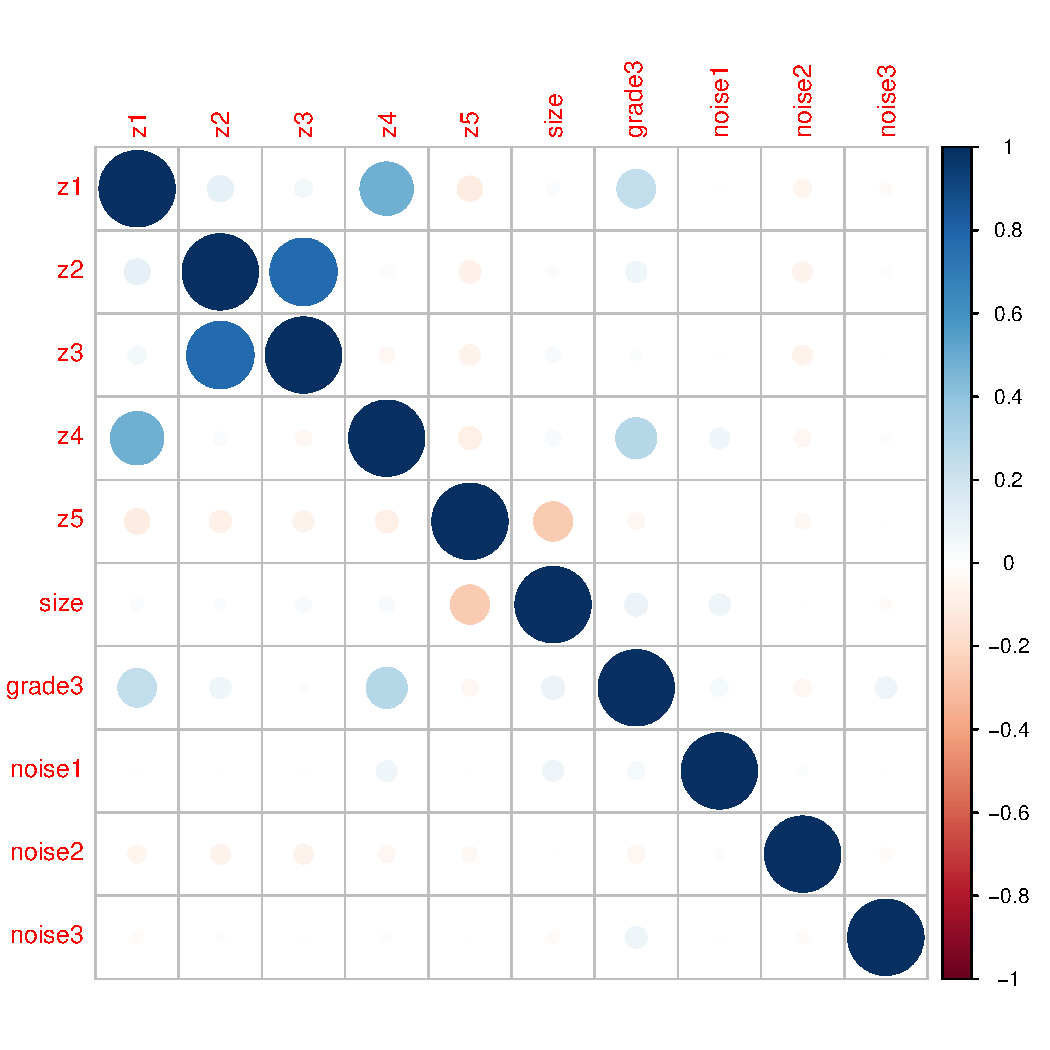
\includegraphics[width=\maxwidth]{figure/r_FSanalysis-2} 
\begin{kframe}\begin{alltt}
\hlcom{# Options Allconfounders.name is list of confounders within analysis dataset}
\hlcom{# (1) use_lasso=TRUE & use_grf=FALSE Lasso used to possibly reduce dimension}
\hlcom{# Any continuous factors are cut at medians (2) use_lasso=TRUE & use_grf=TRUE}
\hlcom{# Lasso used to reduce dimension Continuous covariates are cut at medians}
\hlcom{# However, if GRF selects a covariate cut then only that cut is used: For}
\hlcom{# example if 'age <= median(ag)' is called for per Lasso but GRF includes 'age}
\hlcom{# <= 54', then only the latter is used (3) use_grf_only = TRUE (overrides}
\hlcom{# use_lasso and use_grf) Only factors selected via GRF are used (4) use_lasso =}
\hlcom{# F & use_grf =T Median cuts (unless selected via GRF) as in (2) However no}
\hlcom{# possible dimension reduction via lasso All categorical factors included}

\hlstd{use_lasso} \hlkwb{<-} \hlnum{TRUE}
\hlstd{use_grf} \hlkwb{<-} \hlnum{TRUE}
\hlstd{use_grf_only} \hlkwb{<-} \hlnum{FALSE}

\hlstd{fs.est} \hlkwb{<-} \hlkwd{forestsearch}\hlstd{(}\hlkwc{df.analysis} \hlstd{= x,} \hlkwc{Allconfounders.name} \hlstd{= confounders.name,} \hlkwc{details} \hlstd{=} \hlnum{TRUE}\hlstd{,}
    \hlkwc{use_lasso} \hlstd{= use_lasso,} \hlkwc{use_grf} \hlstd{= use_grf,} \hlkwc{use_grf_only} \hlstd{= use_grf_only,} \hlkwc{dmin.grf} \hlstd{=} \hlnum{10}\hlstd{,}
    \hlkwc{frac.tau} \hlstd{=} \hlnum{0.6}\hlstd{,} \hlkwc{conf_force} \hlstd{=} \hlkwa{NULL}\hlstd{,} \hlkwc{outcome.name} \hlstd{= outcome.name,} \hlkwc{treat.name} \hlstd{= treat.name,}
    \hlkwc{event.name} \hlstd{= event.name,} \hlkwc{id.name} \hlstd{= id.name,} \hlkwc{n.min} \hlstd{= nmin.fs,} \hlkwc{hr.threshold} \hlstd{= hr.threshold,}
    \hlkwc{hr.consistency} \hlstd{= hr.consistency,} \hlkwc{fs.splits} \hlstd{= fs.splits,} \hlkwc{d0.min} \hlstd{= d.min,} \hlkwc{d1.min} \hlstd{= d.min,}
    \hlkwc{pstop_futile} \hlstd{= pstop_futile,} \hlkwc{pconsistency.threshold} \hlstd{= pconsistency.threshold,}
    \hlkwc{stop.threshold} \hlstd{= stop.threshold,} \hlkwc{max.minutes} \hlstd{= max.minutes,} \hlkwc{maxk} \hlstd{= maxk,} \hlkwc{by.risk} \hlstd{=} \hlnum{12}\hlstd{,}
    \hlkwc{plot.sg} \hlstd{=} \hlnum{TRUE}\hlstd{,} \hlkwc{vi.grf.min} \hlstd{= vi.grf.min)}
\end{alltt}
\begin{verbatim}
## tau, maxdepth= 49.69171 2 
##   leaf.node control.mean control.size control.se treated.mean treated.size
## 1         2    -5.156029   413.000000   1.419432     5.156029   413.000000
## 2         3     1.882604   287.000000   1.735410    -1.882604   287.000000
## 3         4    -5.630643   204.000000   2.071336     5.630643   204.000000
## 4         5     5.629364   152.000000   2.514496    -5.629364   152.000000
## 5         6    -4.649491   332.000000   1.494023     4.649491   332.000000
##   treated.se       diff Nsg depth
## 1   1.419432 -10.312058 413     1
## 2   1.735410   3.765209 287     1
## 3   2.071336 -11.261285 204     2
## 4   2.514496  11.258728 152     2
## 5   1.494023  -9.298982 332     2
##   leaf.node control.mean control.size control.se treated.mean treated.size
## 4         5     5.629364   152.000000   2.514496    -5.629364   152.000000
##   treated.se     diff Nsg depth
## 4   2.514496 11.25873 152     2
## [1] "noise2 <= -0.08" "z3 <= 0"         "noise3 <= 1.7"  
## [1] "z3 <= 0"
## # of continuous/categorical characteristics 4 6 
## Continuous characteristics: size noise1 noise2 noise3 
## Categorical characteristics: z1 z2 z3 z4 z5 grade3 
## 10 x 1 sparse Matrix of class "dgCMatrix"
##                  s0
## z1      .          
## z2      .          
## z3      0.112025756
## z4      0.761514747
## z5     -0.863449482
## size    .          
## grade3  .          
## noise1  0.001887115
## noise2  .          
## noise3  .          
## Cox-LASSO selected: z3 z4 z5 noise1 
## Cox-LASSO not selected: z1 z2 size grade3 noise2 noise3 
## Median cuts (after Lasso if use_lasso) noise1 
## Categorical (after Lasso if use_lasso) z3 z4 z5 
## Prior to removing (if in GRF): noise1 
## Left (to cut at median) after removing others if in GRF: noise1 
## Initial GRF cuts included noise2 <= -0.08 z3 <= 0 noise3 <= 1.7 
## # of candidate subgroup factors= 6 
## [1] "noise1 <= median(noise1)" "noise2 <= -0.08"         
## [3] "noise3 <= 1.7"            "z3"                      
## [5] "z4"                       "z5"                      
## Confounders per grf screening q4 q2 q6 q1 q5 
##   FSconfounders.name        vi.cs    vi_ratio
## 4                 q4 0.3456293701 2.073776221
## 2                 q2 0.1907045970 1.144227582
## 6                 q6 0.1713741995 1.028245197
## 1                 q1 0.1558734452 0.935240671
## 5                 q5 0.1360668172 0.816400903
## 3                 q3 0.0003515711 0.002109426
## Number of unique levels (L) and possible subgroups= 10 1023 
## # of subgroups based on # variables > k.max and excluded (per million) 0.000968 
## k.max= 2 
## Events criteria for control,exp= 10 10 
## # of subgroups with events less than criteria: control, experimental 5 5 
## # of subgroups with sample size less than criteria 5 
## # of subgroups meeting all criteria = 50 
## # of subgroups fitted (Cox model estimable) = 50 
## *Subgroup Searching Minutes=* 0.00215 
## Number of subgroups meeting HR threshold 1 
## # of candidate subgroups (meeting HR criteria) =  1 
## Subgroups (1st 10) meeting overall screening thresholds (HR, m1) sorted by HRs= Inf 
##      K   n  E d1    m1    m0   HR L(HR) U(HR) q4.0 q4.1 q2.0 q2.1 q6.0 q6.1
##  1:  2 123 96 44 22.18 44.78 1.64  1.09  2.46    0    1    0    0    0    0
##  2: NA  NA NA NA    NA    NA   NA    NA    NA   NA   NA   NA   NA   NA   NA
##  3: NA  NA NA NA    NA    NA   NA    NA    NA   NA   NA   NA   NA   NA   NA
##  4: NA  NA NA NA    NA    NA   NA    NA    NA   NA   NA   NA   NA   NA   NA
##  5: NA  NA NA NA    NA    NA   NA    NA    NA   NA   NA   NA   NA   NA   NA
##  6: NA  NA NA NA    NA    NA   NA    NA    NA   NA   NA   NA   NA   NA   NA
##  7: NA  NA NA NA    NA    NA   NA    NA    NA   NA   NA   NA   NA   NA   NA
##  8: NA  NA NA NA    NA    NA   NA    NA    NA   NA   NA   NA   NA   NA   NA
##  9: NA  NA NA NA    NA    NA   NA    NA    NA   NA   NA   NA   NA   NA   NA
## 10: NA  NA NA NA    NA    NA   NA    NA    NA   NA   NA   NA   NA   NA   NA
##     q1.0 q1.1 q5.0 q5.1
##  1:    0    0    0    1
##  2:   NA   NA   NA   NA
##  3:   NA   NA   NA   NA
##  4:   NA   NA   NA   NA
##  5:   NA   NA   NA   NA
##  6:   NA   NA   NA   NA
##  7:   NA   NA   NA   NA
##  8:   NA   NA   NA   NA
##  9:   NA   NA   NA   NA
## 10:   NA   NA   NA   NA
## Consistency 0.9775 
## # of splits= 400 
## Model, % Consistency Met= {z3} {z4} 0.9775 
## Number of subgroups meeting consistency criteria= 
##    p.consistency Nsg group.id m.index K  M.1  M.2
## 1:        0.9775 123        1       1 2 {z3} {z4}
\end{verbatim}
\end{kframe}
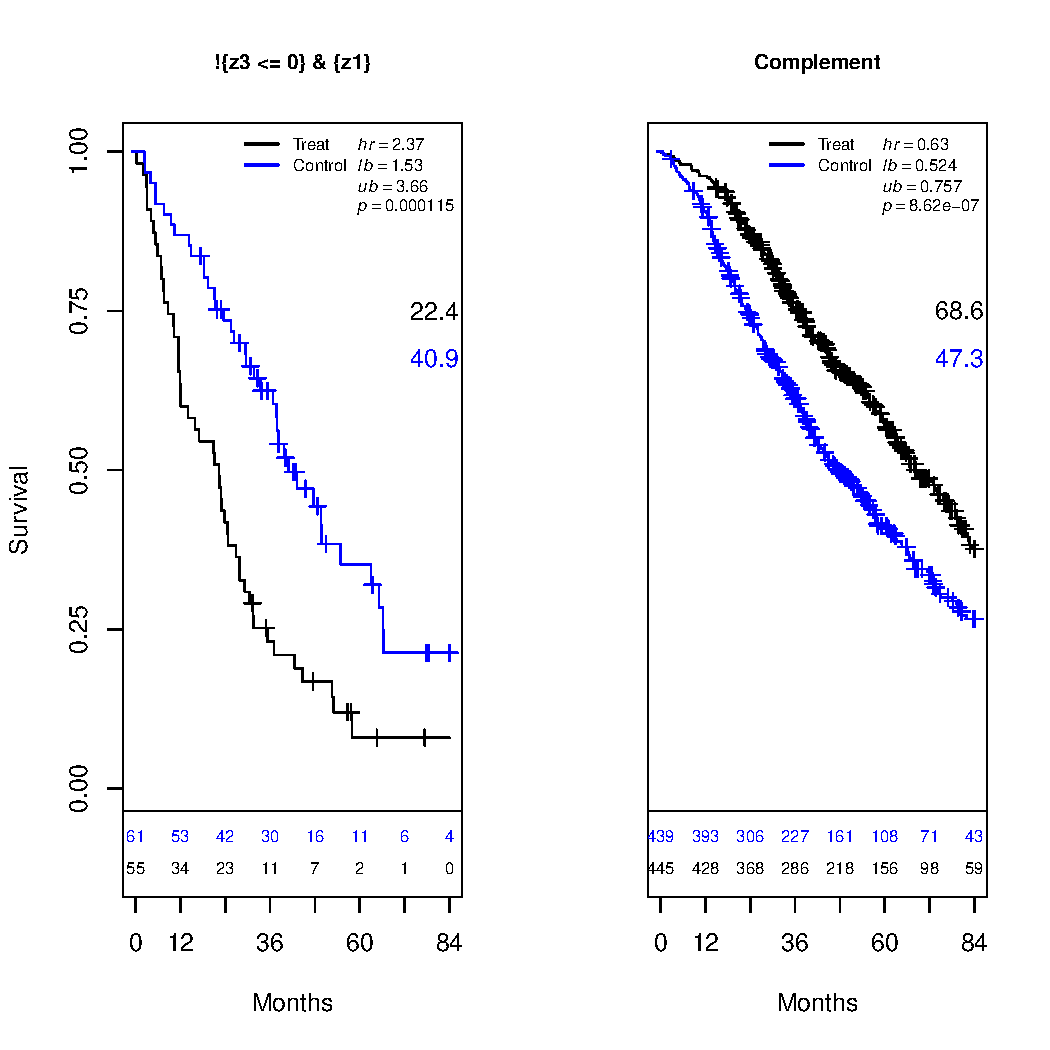
\includegraphics[width=\maxwidth]{figure/r_FSanalysis-3} 
\begin{kframe}\begin{verbatim}
## [1] "{z3}" "{z4}"
## % consistency criteria met= 0.9775 
## SG focus= hr 
## Subgroup Consistency Minutes= 0.0264 
## Subgroup found 
## Minutes overall= 0.04795
\end{verbatim}
\begin{alltt}
\hlstd{grf.est} \hlkwb{<-} \hlkwd{grf.subg.harm.survival}\hlstd{(}\hlkwc{data} \hlstd{= x,} \hlkwc{confounders.name} \hlstd{= confounders.name,}
    \hlkwc{outcome.name} \hlstd{= outcome.name,} \hlkwc{event.name} \hlstd{= event.name,} \hlkwc{id.name} \hlstd{= id.name,} \hlkwc{treat.name} \hlstd{= treat.name,}
    \hlkwc{n.min} \hlstd{= n.min,} \hlkwc{dmin.grf} \hlstd{= dmin.grf,} \hlkwc{frac.tau} \hlstd{=} \hlnum{1}\hlstd{,} \hlkwc{details} \hlstd{=} \hlnum{TRUE}\hlstd{)}
\end{alltt}
\begin{verbatim}
## tau, maxdepth= 82.81952 2 
##    leaf.node control.mean control.size control.se treated.mean treated.size
## 1          2    -9.865316   537.000000   2.271331     9.865316   537.000000
## 2          3     1.431633   163.000000   4.189690    -1.431633   163.000000
## 11         4    -9.421142   520.000000   2.287215     9.421142   520.000000
## 3          6   -16.120361    96.000000   5.206166    16.120361    96.000000
## 4          7    15.311287    79.000000   6.179571   -15.311287    79.000000
##    treated.se       diff Nsg depth
## 1    2.271331 -19.730633 537     1
## 2    4.189690   2.863266 163     1
## 11   2.287215 -18.842283 520     2
## 3    5.206166 -32.240722  96     2
## 4    6.179571  30.622574  79     2
##   leaf.node control.mean control.size control.se treated.mean treated.size
## 4         7    15.311287    79.000000   6.179571   -15.311287    79.000000
##   treated.se     diff Nsg depth
## 4   6.179571 30.62257  79     2
## [1] "z1 <= 0"    "size <= 80" "z3 <= 0"   
## [1] "z3 <= 0"
\end{verbatim}
\end{kframe}
\end{knitrout}


\begin{knitrout}
\definecolor{shadecolor}{rgb}{0.969, 0.969, 0.969}\color{fgcolor}\begin{kframe}
\begin{alltt}
\hlkwd{library}\hlstd{(doParallel)}
\hlkwd{registerDoParallel}\hlstd{(parallel}\hlopt{::}\hlkwd{detectCores}\hlstd{(}\hlkwc{logical} \hlstd{=} \hlnum{FALSE}\hlstd{))}

\hlstd{cox.formula.boot} \hlkwb{<-} \hlstd{cox.formula.sim}
\hlstd{max.minutes} \hlkwb{<-} \hlnum{7}
\hlcom{# Suggest running 50, first ... to get timing estimate}

\hlstd{NB} \hlkwb{<-} \hlnum{1000}

\hlstd{df_boot_analysis} \hlkwb{<-} \hlstd{fs.est}\hlopt{$}\hlstd{df.est}

\hlstd{fitH} \hlkwb{<-} \hlkwd{get_Cox_sg}\hlstd{(}\hlkwc{df_sg} \hlstd{=} \hlkwd{subset}\hlstd{(df_boot_analysis, treat.recommend} \hlopt{==} \hlnum{0}\hlstd{),} \hlkwc{cox.formula} \hlstd{= cox.formula.boot)}
\hlstd{H_obs} \hlkwb{<-} \hlstd{fitH}\hlopt{$}\hlstd{est_obs}  \hlcom{# log(hr) scale}
\hlstd{seH_obs} \hlkwb{<-} \hlstd{fitH}\hlopt{$}\hlstd{se_obs}
\hlcom{# Hc observed estimates}
\hlstd{fitHc} \hlkwb{<-} \hlkwd{get_Cox_sg}\hlstd{(}\hlkwc{df_sg} \hlstd{=} \hlkwd{subset}\hlstd{(df_boot_analysis, treat.recommend} \hlopt{==} \hlnum{1}\hlstd{),} \hlkwc{cox.formula} \hlstd{= cox.formula.boot)}
\hlstd{Hc_obs} \hlkwb{<-} \hlstd{fitHc}\hlopt{$}\hlstd{est_obs}
\hlstd{seHc_obs} \hlkwb{<-} \hlstd{fitHc}\hlopt{$}\hlstd{se_obs}
\hlkwd{rm}\hlstd{(}\hlstr{"fitH"}\hlstd{,} \hlstr{"fitHc"}\hlstd{)}

\hlstd{Ystar_mat} \hlkwb{<-} \hlkwd{bootYstar}\hlstd{(\{}
    \hlstd{ystar} \hlkwb{<-} \hlkwd{get_Ystar}\hlstd{(boot)}
\hlstd{\},} \hlkwc{boots} \hlstd{= NB,} \hlkwc{seed} \hlstd{=} \hlnum{8316951}\hlstd{,} \hlkwc{counter} \hlstd{=} \hlstr{"boot"}\hlstd{,} \hlkwc{export} \hlstd{= fun_arg_list_boot)}
\hlcom{# Check dimension}
\hlkwa{if} \hlstd{(}\hlkwd{dim}\hlstd{(Ystar_mat)[}\hlnum{1}\hlstd{]} \hlopt{!=} \hlstd{NB} \hlopt{|} \hlkwd{dim}\hlstd{(Ystar_mat)[}\hlnum{2}\hlstd{]} \hlopt{!=} \hlkwd{nrow}\hlstd{(df_boot_analysis))} \hlkwd{stop}\hlstd{(}\hlstr{"Dimension of Ystar_mat does not match"}\hlstd{)}

\hlstd{tB.start} \hlkwb{<-} \hlkwd{proc.time}\hlstd{()[}\hlnum{3}\hlstd{]}
\hlcom{# Bootstraps}
\hlstd{resB} \hlkwb{<-} \hlkwd{bootPar}\hlstd{(\{}
    \hlstd{ans} \hlkwb{<-} \hlkwd{fsboot_forparallel}\hlstd{(boot)}
\hlstd{\},} \hlkwc{boots} \hlstd{= NB,} \hlkwc{seed} \hlstd{=} \hlnum{8316951}\hlstd{,} \hlkwc{counter} \hlstd{=} \hlstr{"boot"}\hlstd{,} \hlkwc{export} \hlstd{= fun_arg_list_boot)}
\hlstd{tB.now} \hlkwb{<-} \hlkwd{proc.time}\hlstd{()[}\hlnum{3}\hlstd{]}
\hlstd{tB.min} \hlkwb{<-} \hlstd{(tB.now} \hlopt{-} \hlstd{tB.start)}\hlopt{/}\hlnum{60}

\hlstd{doParallel}\hlopt{::}\hlkwd{stopImplicitCluster}\hlstd{()}

\hlkwd{cat}\hlstd{(}\hlstr{"Minutes for Boots"}\hlstd{,} \hlkwd{c}\hlstd{(NB, tB.min),} \hlstr{"\textbackslash{}n"}\hlstd{)}
\end{alltt}
\begin{verbatim}
## Minutes for Boots 1000 3.588317
\end{verbatim}
\begin{alltt}
\hlkwd{cat}\hlstd{(}\hlstr{"Projection per 1000"}\hlstd{,} \hlkwd{c}\hlstd{(tB.min} \hlopt{*} \hlstd{(}\hlnum{1000}\hlopt{/}\hlstd{NB)),} \hlstr{"\textbackslash{}n"}\hlstd{)}
\end{alltt}
\begin{verbatim}
## Projection per 1000 3.588317
\end{verbatim}
\begin{alltt}
\hlkwd{cat}\hlstd{(}\hlstr{"Propn bootstrap subgroups found ="}\hlstd{,} \hlkwd{c}\hlstd{(}\hlkwd{sum}\hlstd{(}\hlopt{!}\hlkwd{is.na}\hlstd{(resB}\hlopt{$}\hlstd{H_biasadj_1))}\hlopt{/}\hlstd{NB),} \hlstr{"\textbackslash{}n"}\hlstd{)}
\end{alltt}
\begin{verbatim}
## Propn bootstrap subgroups found = 0.945
\end{verbatim}
\begin{alltt}
\hlcom{# How many timmed out}
\hlkwd{cat}\hlstd{(}\hlstr{"Number timmed out="}\hlstd{,} \hlkwd{c}\hlstd{(}\hlkwd{sum}\hlstd{(}\hlkwd{is.na}\hlstd{(resB}\hlopt{$}\hlstd{H_biasadj_1)} \hlopt{&} \hlstd{resB}\hlopt{$}\hlstd{tmins_search} \hlopt{>} \hlstd{max.minutes)),}
    \hlstr{"\textbackslash{}n"}\hlstd{)}
\end{alltt}
\begin{verbatim}
## Number timmed out= 0
\end{verbatim}
\begin{alltt}
\hlstd{H_estimates} \hlkwb{<-} \hlkwd{get_dfRes}\hlstd{(}\hlkwc{Hobs} \hlstd{= H_obs,} \hlkwc{seHobs} \hlstd{= seH_obs,} \hlkwc{H1_adj} \hlstd{= resB}\hlopt{$}\hlstd{H_biasadj_2,}
    \hlkwc{ystar} \hlstd{= Ystar_mat,} \hlkwc{cov_method} \hlstd{=} \hlstr{"standard"}\hlstd{,} \hlkwc{cov_trim} \hlstd{=} \hlnum{0}\hlstd{)}
\hlstd{Hc_estimates} \hlkwb{<-} \hlkwd{get_dfRes}\hlstd{(}\hlkwc{Hobs} \hlstd{= Hc_obs,} \hlkwc{seHobs} \hlstd{= seHc_obs,} \hlkwc{H1_adj} \hlstd{= resB}\hlopt{$}\hlstd{Hc_biasadj_2,}
    \hlkwc{ystar} \hlstd{= Ystar_mat,} \hlkwc{cov_method} \hlstd{=} \hlstr{"standard"}\hlstd{,} \hlkwc{cov_trim} \hlstd{=} \hlnum{0}\hlstd{)}

\hlkwd{print}\hlstd{(H_estimates)}
\end{alltt}
\begin{verbatim}
##          H0      sdH0 H0_lower H0_upper       H1     sdH1  H1_lower H1_upper
## 1: 1.639708 0.3378324 1.094943 2.455508 1.408539 0.380832 0.8291373 2.392828
\end{verbatim}
\begin{alltt}
\hlkwd{print}\hlstd{(Hc_estimates)}
\end{alltt}
\begin{verbatim}
##           H0      sdH0  H0_lower  H0_upper        H1      sdH1  H1_lower
## 1: 0.5909388 0.0719693 0.4654535 0.7502546 0.6004953 0.1132946 0.4148724
##     H1_upper
## 1: 0.8691698
\end{verbatim}
\begin{alltt}
\hlcom{# H_estimates<-get_dfRes(Hobs=H_obs,seHobs=seH_obs,H1_adj=resB$H_biasadj_1,ystar=Ystar_mat,cov_method='standard',cov_trim=0.025)}
\hlcom{# Hc_estimates<-get_dfRes(Hobs=Hc_obs,seHobs=seHc_obs,H1_adj=resB$Hc_biasadj_1,ystar=Ystar_mat,cov_method='standard',cov_trim=0.025)}
\hlcom{# print(H_estimates) print(Hc_estimates)}


\hlstd{bootit} \hlkwb{<-} \hlkwd{list}\hlstd{(}\hlkwc{H_estimates} \hlstd{= H_estimates,} \hlkwc{Hc_estimates} \hlstd{= Hc_estimates)}
\hlstd{ans3} \hlkwb{<-} \hlkwd{fsBoot.parallel.out}\hlstd{(}\hlkwc{df} \hlstd{= df_boot_analysis,} \hlkwc{FSboots} \hlstd{= bootit,} \hlkwc{cox.formula.boot} \hlstd{= cox.formula.boot,}
    \hlkwc{sim_number} \hlstd{= sim)}
\hlstd{tall.min} \hlkwb{<-} \hlstd{(tB.now} \hlopt{-} \hlstd{t.start.all)}\hlopt{/}\hlnum{60}
\hlkwd{cat}\hlstd{(}\hlstr{"Overall minutes for analysis"}\hlstd{,} \hlkwd{c}\hlstd{(tall.min),} \hlstr{"\textbackslash{}n"}\hlstd{)}
\end{alltt}
\begin{verbatim}
## Overall minutes for analysis 3.716533
\end{verbatim}
\begin{alltt}
\hlkwd{save}\hlstd{(dgm, x, fs.est, grf.est, bootit, ans3, tall.min, resB, cox.formula.boot,} \hlkwc{file} \hlstd{= file_out)}

\hlcom{# ITT causal hazard ratio mean(fs.est$df.est$hlin.ratio) H Oracle dfH <-}
\hlcom{# subset(fs.est$df.est, flag.harm==1) mean(dfH$hlin.ratio) dfH_est <-}
\hlcom{# subset(fs.est$df.est, treat.recommend==0) mean(dfH_est$hlin.ratio) dfHc <-}
\hlcom{# subset(fs.est$df.est, flag.harm==0) mean(dfHc$hlin.ratio) dfHc_est <-}
\hlcom{# subset(fs.est$df.est, treat.recommend==1) mean(dfHc_est$hlin.ratio)}

\hlcom{# dfSens <- subset(fs.est$df.est, flag.harm==1 & treat.recommend==0) sensH <-}
\hlcom{# nrow(dfSens)/nrow(dfH)}
\end{alltt}
\end{kframe}
\end{knitrout}



\begin{knitrout}
\definecolor{shadecolor}{rgb}{0.969, 0.969, 0.969}\color{fgcolor}\begin{kframe}
\begin{verbatim}
## Confounders evaluated in Forestsearch:
## [1] "noise1 <= median(noise1)" "noise2 <= -0.08"         
## [3] "noise3 <= 1.7"            "z3"                      
## [5] "z4"                       "z5"
\end{verbatim}
\end{kframe}
\end{knitrout}





\begin{table}

\caption{\label{tab:simex_tab}\label{tab:simex} Simulated data example: Cox hazard ratio (hr) estimates for the ITT population and subgroups $H$ and $H^{c}$.
Cox model estimates are based on subgroups: H true (knowing the actual subgroup, a-priori); the estimated subgroup $\hat{H}$; and 
the boostrap ($1,000$ resamples) bias-correction to $\hat{H}$ estimates, denoted $\hat{H}_{bc}$.  Estimates for the complement $H^{c}$ are defined analogously.
The number of subjects in each population ($\#$ Subjects) and the number of subjects correctly classified ($\#$ Correct) in the true subgroups $H$ and $H^{c}$, respectively, are listed.}
\centering
\fontsize{9}{11}\selectfont
\begin{tabular}[t]{lccccc}
\toprule
  & HR Estimate & Lower & Upper & $\#$ Subjects & $\#$ Correct\\
\midrule
ITT & 0.691 & 0.563 & 0.849 & 700 & .\\
\addlinespace[0.3em]
\multicolumn{6}{l}{\textbf{H subgroup estimates}}\\
\hspace{1em}$H_{oracle}$ & 3.456 & 2.049 & 5.83 & 79 & .\\
\hspace{1em}$\hat{H}$ & 1.64 & 1.095 & 2.456 & 123 & 64\\
\hspace{1em}$\hat{H}_{bc}$ & 1.409 & 0.829 & 2.394 & 123 & 64\\
\addlinespace[0.3em]
\multicolumn{6}{l}{\textbf{H-complement subgroup estimates}}\\
\hspace{1em}$H^{c}_{oracle}$ & 0.601 & 0.48 & 0.753 & 621 & .\\
\hspace{1em}$\hat{H}^{c}$ & 0.591 & 0.465 & 0.75 & 577 & 562\\
\hspace{1em}$\hat{H}^{c}_{bc}$ & 0.6 & 0.415 & 0.868 & 577 & 562\\
\bottomrule
\end{tabular}
\end{table}




\bibliographystyle{spbasic}      % basic style, author-year citations
\bibliography{../../subgroups_ref}
\end{document}
